\documentclass{beamer}
%\usecolortheme{seahorse} % change this
\usepackage{graphicx}
\usepackage{inconsolata}
\usepackage{anyfontsize}
\usepackage{courier}
\usepackage{color}


\usepackage{natbib} 
%bibstyle muss einer da sein, 
% setimmt wie der kram an \cite aussieht.
% https://de.wikibooks.org/wiki/LaTeX-W%C3%B6rterbuch:_bibliographystyle
%https://de.sharelatex.com/learn/Bibtex_bibliography_styles
%\bibliographystyle{abbrvnat} 
%\bibliographystyle{unsrt} 
\bibliographystyle{plainnat}

%gets rid of bottom navigation bars
\setbeamertemplate{footline}[frame number]{}

%gets rid of bottom navigation symbols
\setbeamertemplate{navigation symbols}{}

%gets rid of footer
%will override 'frame number' instruction above
%comment out to revert to previous/default definitions
\setbeamertemplate{footline}{}

\newcommand{\red}[1]{\textcolor{red}{#1}}

\title 
{A Constructive Approach for Graph Concepts \\
with Long Range Dependencies}
\author % NEEDS MOAR INFO ,, contact etc
%{Stefan Mautner }
{Fabrizio Costa  \and \underline{Stefan Mautner}
    \small{ 
        \texttt{
            \href{mailto:costa@informatik.uni-freiburg.de}
            {costa@informatik.uni-freiburg.de}}
            \texttt{
            \href{mailto:mautner@informatik.uni-freiburg.de}
            {mautner@informatik.uni-freiburg.de}}
        }
}

\date 
{Freiburg University \\2016-12-09}

\titlegraphic{
\includegraphics[width=2cm]{images/logo.jpg}
}

\begin{document}
\frame{\titlepage}



% design goals
\begin{frame}
\frametitle{Constructive Machine Learning}

    \begin{itemize}
        \item {\bf What:} Answer \red{design} questions using examples
        \item We are interested in: \\generative approaches for \red{structured} domains
        \item Chemo- and bio-informatics: \\synthesize molecules with a desired bioactivity
    \end{itemize}
    \begin{figure}
        \centering
        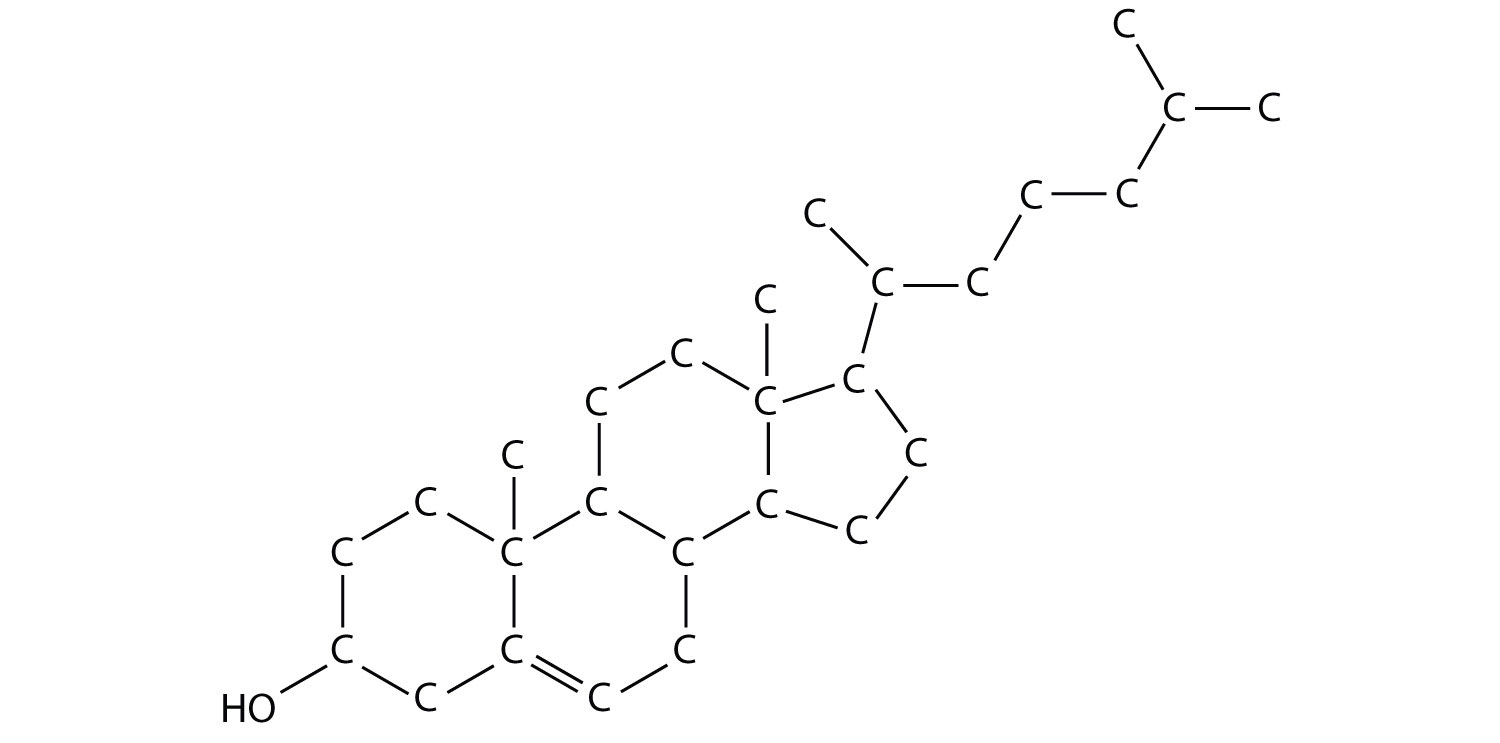
\includegraphics[width=0.5\textwidth]{images/mol.jpg}
        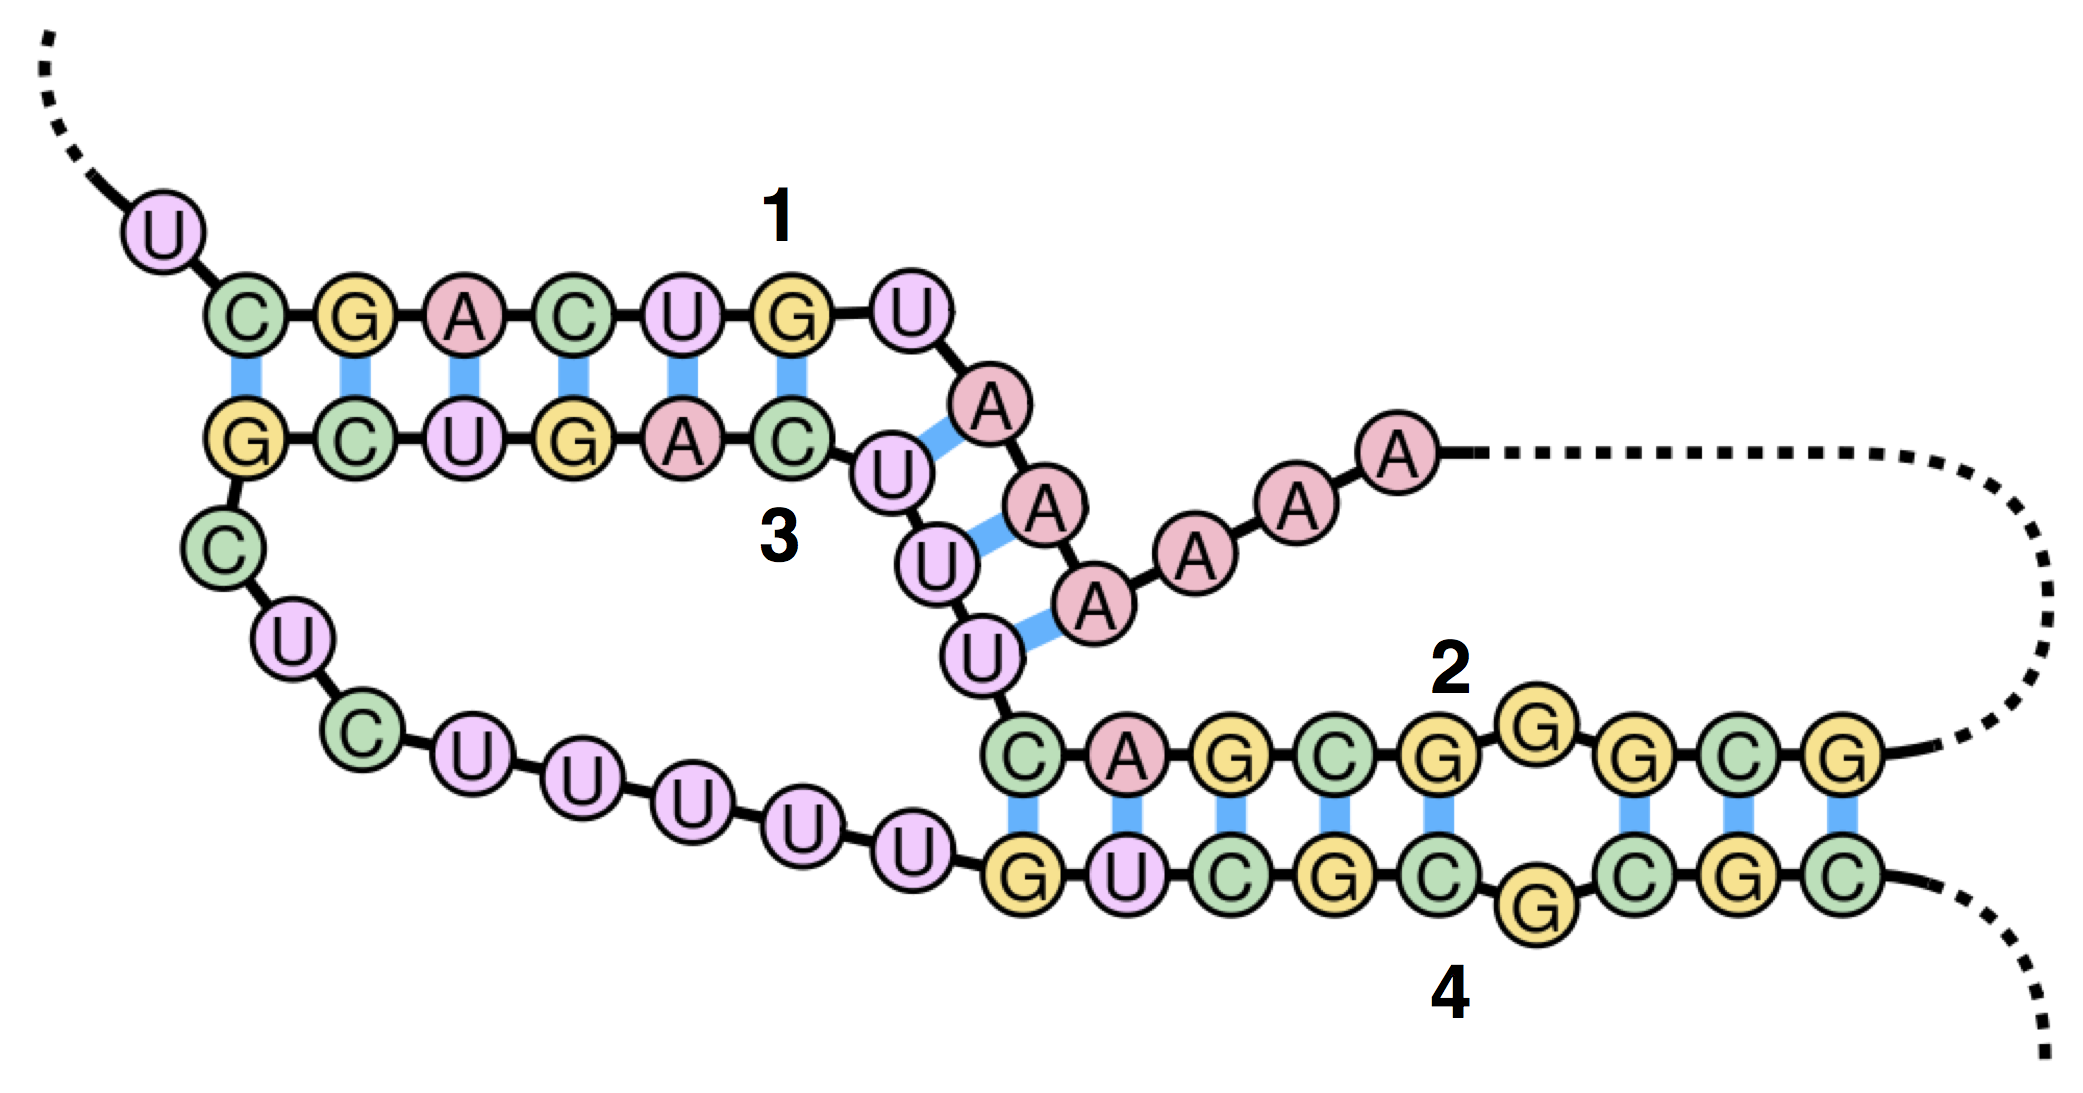
\includegraphics[width=0.5\textwidth]{images/rna.png}
    \end{figure}    
\end{frame}

\begin{frame}
\frametitle{Constructive Machine Learning}

    \begin{itemize}
        \item Molecules can have complex dependencies between {\em parts}
        \item RNA self interact: bounds that span the entire length
        \item Modeling long range dependencies is \red{hard}
        \item Our proposal:\\ long range $\mapsto$ short range in \red{coarse} representation
    \end{itemize}
    \begin{figure}[ht]
        \centering
        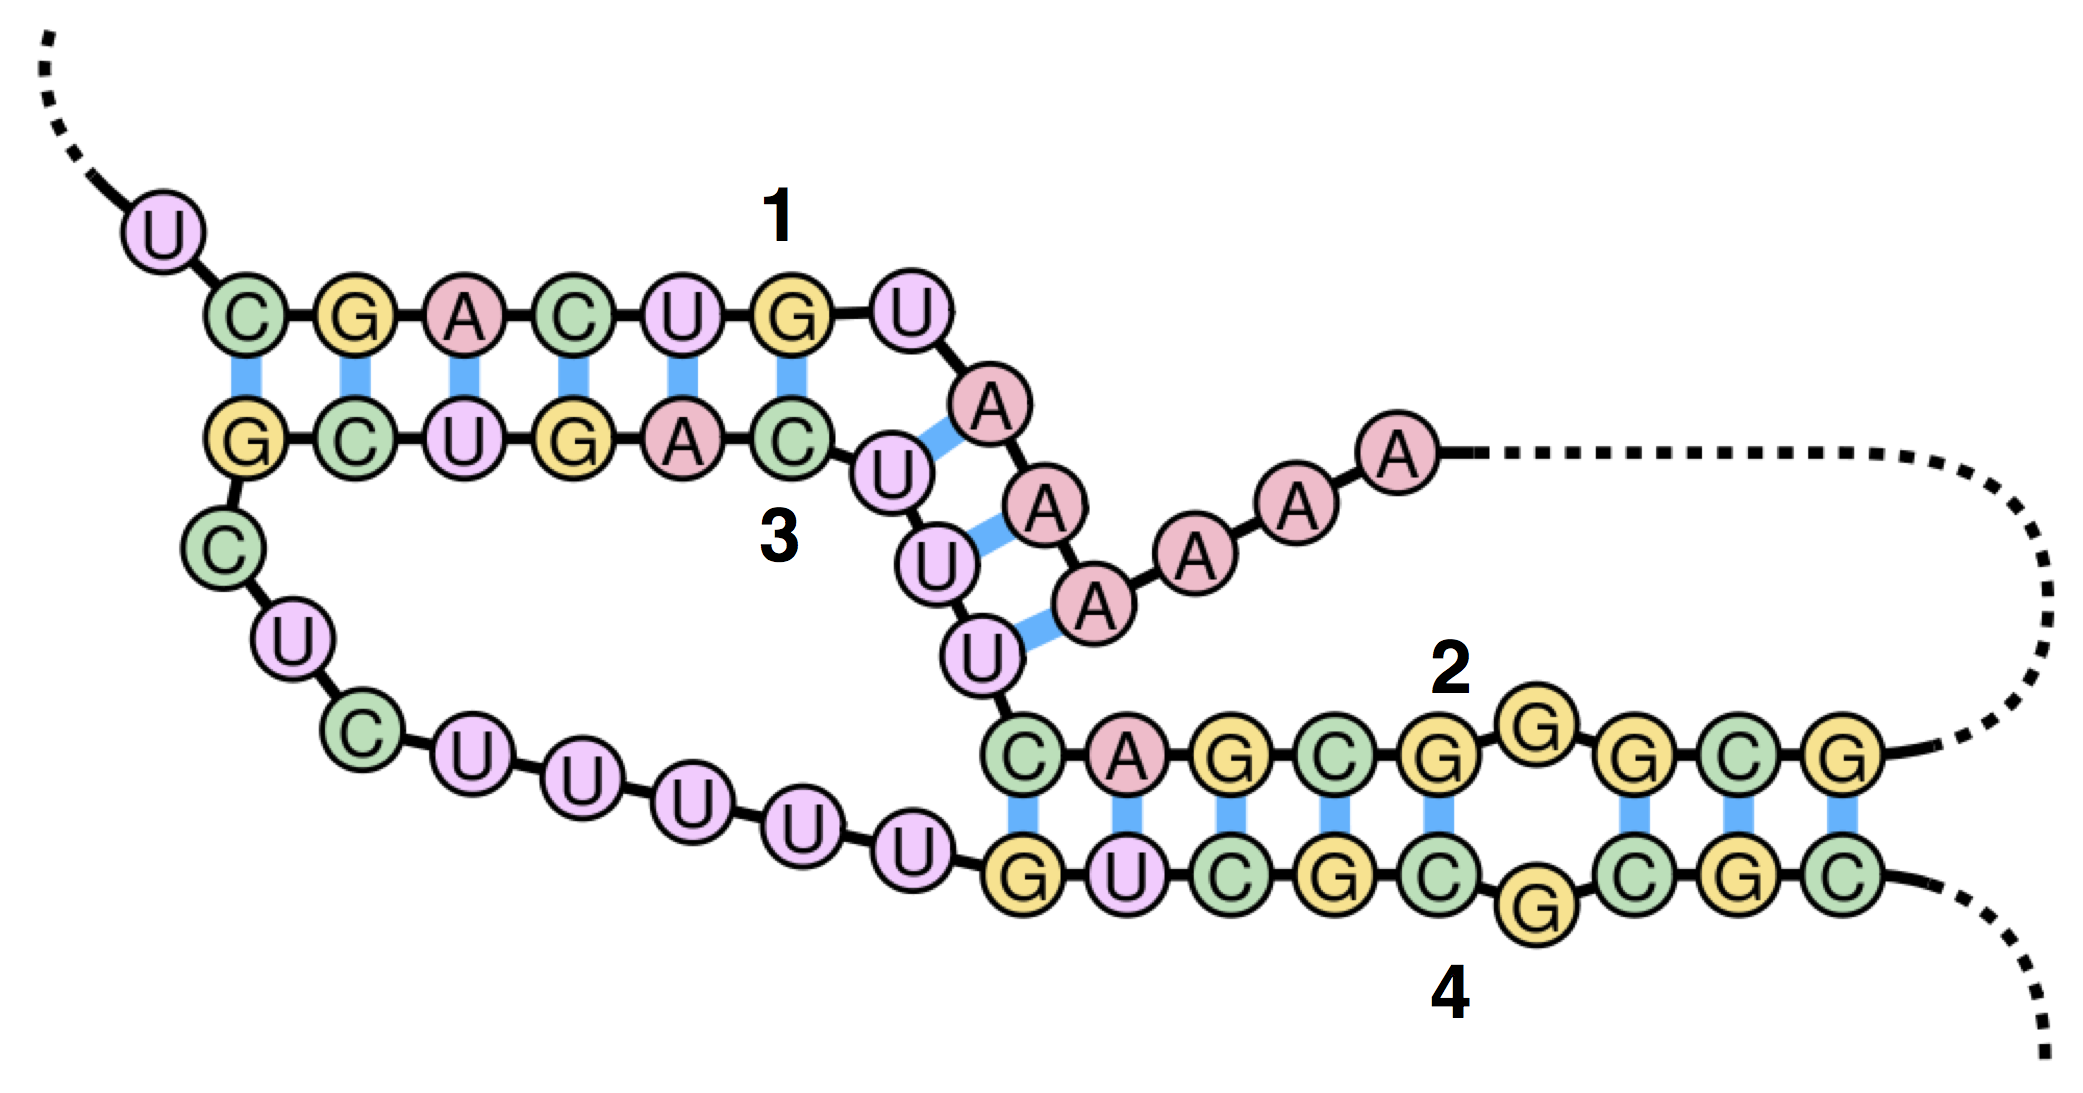
\includegraphics[width=0.7\textwidth]{images/rna.png}
    \end{figure}    
\end{frame}

\begin{frame}
\frametitle{The constructive learning problem for finite samples\footnote{Costa Artif. Intell. 2016}}
    \begin{itemize}
        \item Given a set of graphs $G$
        \item use a parametrized generator $M_\theta$ to \red{construct} $G_\theta$
        \item find optimal $\theta$ to \red{jointly} satisfy:
            \begin{enumerate}
        \item probability density is the \red{same} if estimated over $G$ or $G_\theta$
        \item generated graphs $G_\theta$ are \red{different} from originals $G$
            \end{enumerate}
        \item Optimize:\\ \begin{center} $\arg \min_\theta L(P(G),P(G_\theta)) + \lambda  ~ Sim(G, G_\theta)$ \end{center}
        \item where:
        \begin{itemize}
            \item $L$ is a loss over probability distributions \\(e.g. Kullback Leibler divergence)
            \item $Sim$ is a set graph kernel
        \end{itemize}
    
    \end{itemize}
    %$${argmin}_{\theta}~~L(f_{G_0}(G),f_{G_{\theta}}(G))+\lambda \frac{K(G_0,G_{\theta})}{\sqrt{K(G_0,G_0),K(G_{\theta},G_{\theta})}}}$$
\end{frame}


% so far we have the basic graphlearn
\begin{frame}
    \frametitle{Parametrized Generator for Graphs}
    \begin{itemize}
        \item Instead of generating $\mapsto$ \red{sample} from a corresponding underlying probability distribution over graphs
        \item We use a Metropolis Hastings (MH) Markov Chain Monte Carlo (MCMC) method
        \begin{enumerate}
            \item start from {\em seed} graph $x$
            \item proposal distribution $g(x \mapsto x')$
            \item accept with acceptance prob: \\
            \begin{center}
            $A(x \mapsto x')=\min(1, \frac{P(x')}{P(x)} \frac{g(x \mapsto x')}{g(x' \mapsto x)})$
            \end{center}
        \end{enumerate}
        \item {\bf Q:} How to propose new graphs?
        \item {\bf A:} use graph \red{grammar}
    \end{itemize}
\end{frame}

\begin{frame}
    \frametitle{Graph Grammar}
    A graph grammar is a finite set of productions P=(M,D,E)

    \begin{itemize}
        \item M=mother graph
        \item D=daughter graph
        \item E=embedding mechanism
    \end{itemize}
    \begin{figure}[ht]
        \centering
        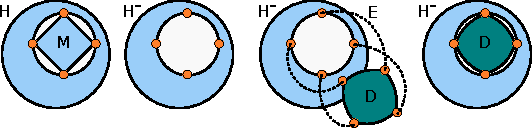
\includegraphics[width=0.9\textwidth]{images/grammar.pdf}
    \end{figure}
\end{frame}

\begin{frame}
    \frametitle{Substitutable Graph Grammar}
    \begin{itemize}
        \item \red{cores} (neighborhood graphs) can be substituted 

        \item if they have the same \red{interface} graph
    \end{itemize}
    \begin{figure}[ht]
        \centering
        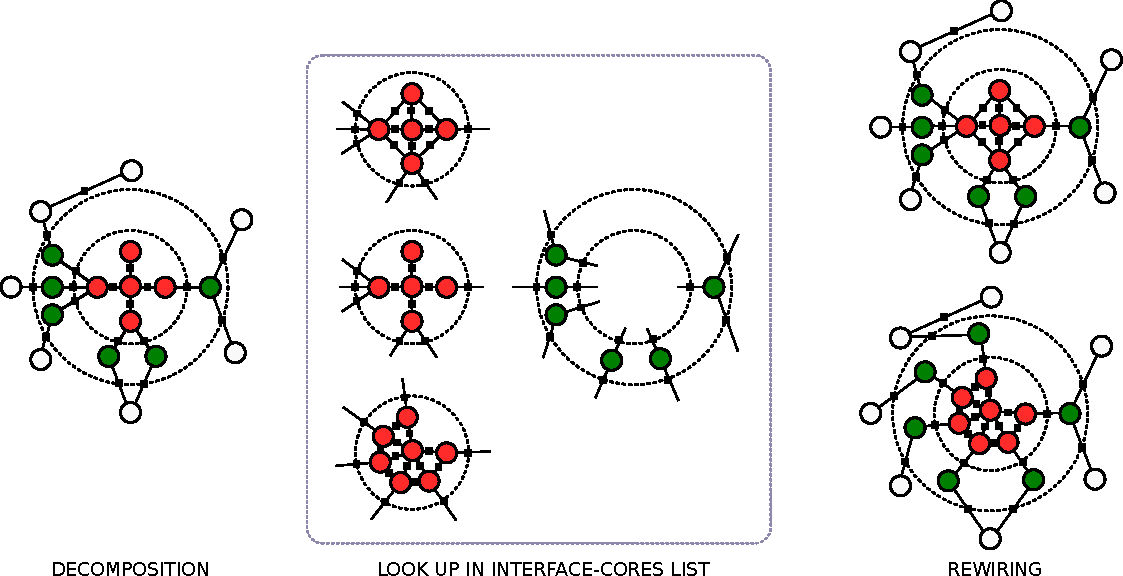
\includegraphics[width=0.9\textwidth]{images/cip.pdf}
    \end{figure}
\end{frame}




% problem with RNA 
\begin{frame}
    \frametitle{Long range dependencies}
    When graphs become larger..
    \begin{itemize}
        \item $\exists$ dependencies between far apart nodes 
        \item ...but we can afford only \red{small} interface graphs  \\
        {\em exponential num interface graphs with their size} \\
        {\em not enough samples to collect statistics}
    \end{itemize}
   \begin{figure}[h!]
        \centering
        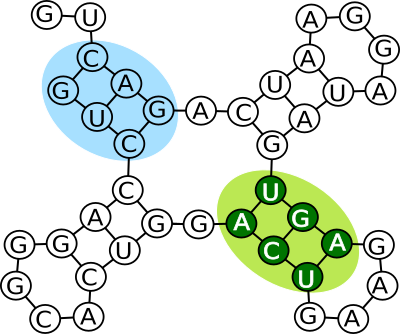
\includegraphics[width=0.45\textwidth]{images/longrangedep.png}
    \end{figure}
    
\end{frame}



% solution
\begin{frame}
    \frametitle{Solution: graph coarsening}
    \begin{itemize}
        \item Allow user defined graph \red{coarsening}:\\
        \red{collapse} selected nodes into a single node
        \item {\em core} is induced by coarse level (dark green)
        \item {\em interface} (light green) is: \\context of core at original level $\times$ context at coarse level
   \end{itemize}
    {\bf Note:} cores are now arbitrarily large\\
    interfaces are small, but model large parts of the graph
   \begin{figure}[ht]
        \centering
        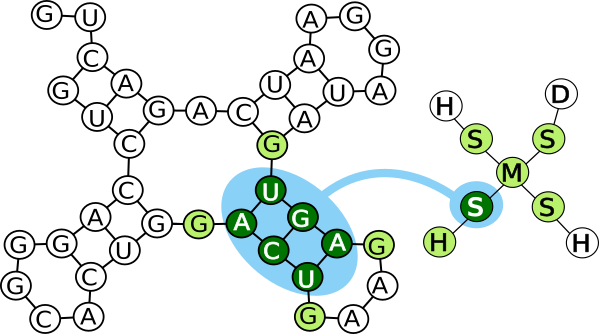
\includegraphics[width=0.50\textwidth]{images/nucip.png}
    \end{figure}
   
\end{frame}





% BENCHMARK I 
\begin{frame}
    \frametitle{Evaluation I}
    \begin{itemize}
        \item Generate RNA sequences with specific \red{function}
        \item RFAM database classifies RNAs with known functions
        \item Covariance model INFERNAL is state-of-the-art RNA classifier 
    \end{itemize}

   \begin{figure}[ht]
        \centering
        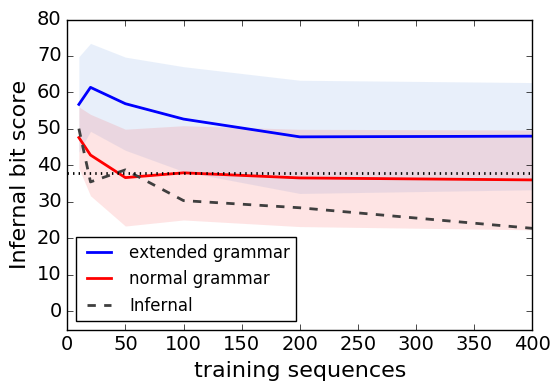
\includegraphics[width=0.70\textwidth]{images/infernal_abstr.png}
    \end{figure}
   \small{\em scores above horizontal dotted line indicate reliable identification}
\end{frame}

% BENCHMARK II
\begin{frame}
    \frametitle{Evaluation II}
    
    \begin{itemize}
        \item {\bf Q:} are generated instances different from originals?
    \end{itemize}
   \begin{figure}[ht]
        \centering
        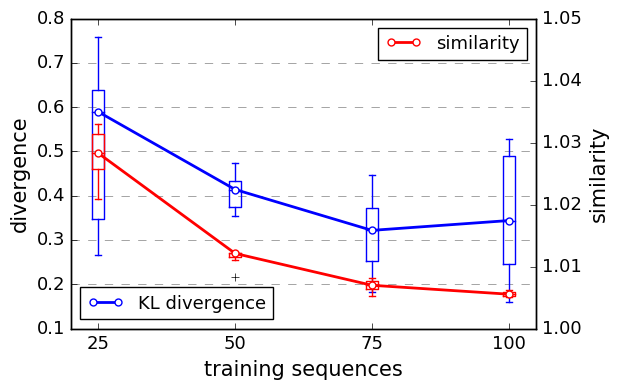
\includegraphics[width=0.85\textwidth]{images/learningcurve.png}
    \end{figure}
\end{frame}

% OWARI DA 
\begin{frame}
    \frametitle{Conclusion}
    
    \begin{itemize}
        \item Coarsening increases expressiveness of graph grammar  
        \item {\bf Future work:} \\learn task specific coarsening strategy directly from data   
    \end{itemize}

    %\begin{itemize}
    %\end{itemize}
\end{frame}


\end{document}
